\newpage
\section{Introduction}
Database: a very large, integrated collection of data. 

Models a real-world enterprise: 
\begin{itemize}
    \item Entities
    \item Relationship
    \item Active components
\end{itemize}

A Database Management System (DBMS) is a software system designed to store, manage and facilitate access to databases. 

\subsection{Purpose of Database Systems}

\subsubsection{Database Applications}
Data processing and management. 

\subsubsection{Several Concepts}
Database

Data Management System (DBMS): database + a set of program. 

Characteristics of DBMS
\begin{itemize}
    \item Efficiency and scalability in \hl{data access}. 
    \item Reduced \hl{application development time}. 
    \item Data \hl{independence} (including \hl{physical data independence} and \hl{logical data independence}).
    \item Data \hl{integrity} and \hl{security}. 
    \item \hl{Concurrent} access and \hl{robustness}. 
\end{itemize}

\subsubsection{File-Processing System}
File-processing system is supported by a conventional Operating System (OS). 

Drawbacks of FPS
\begin{itemize}
    \item Data redundancy and inconsistency. 
    \item Difficulty in accessing data. 
    \item Data isolation --- multiple files and multiple formats. 
    \item Integrity problems. 
    \item No atomicity of updates. 
    \item Difficlut to concurrent access by multiple users. 
    \item Security problems. 
\end{itemize}

\subsection{View of Data}

\subsubsection{Levels of Data Abstraction}

\begin{itemize}
    \item Physical level
    \item Logical level
    \item View level
\end{itemize}

\subsubsection{Schemas and Instance}
Schemas: the structure of the database on different level. 
\begin{itemize}
    \item Physical schema
    \item Logical schema
    \item Subschema
\end{itemize}

Instance: the actual content of the database at a particular point in time. 

\begin{figure}[H]
    \centering
    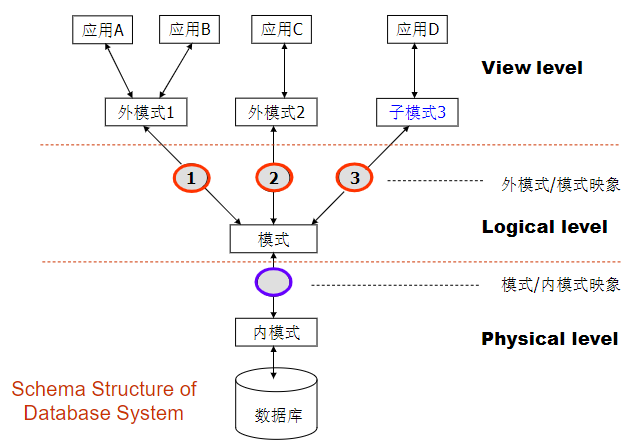
\includegraphics[width=0.309\textwidth]{DB1/Schemas and Instance}
    \caption{Schemas and Instance}
\end{figure}


\subsubsection{Physical Independence vs Logical Independence}
Ability to modify a schema definition at one level without affecting a schema definition at a higher level.
\begin{enumerate}
    \item Physical data independence –-- the ability to modify the physical schema without changing the logical schema.
    \item Logical data independence –-- protect application programs from changes in logical structure of data. 
\end{enumerate}


\subsubsection{Data Models}
Data model is a collection of conceptual for describing. 
\begin{itemize}
    \item data structure
    \item data relationships
    \item data semantics
    \item data constraints
\end{itemize}
Different level of data abstraction needs different data model to describe. 
\begin{itemize}
    \item Entity-Relationship model
    \item Relational model
    \item Other models 
\end{itemize}

\subsection{Database Language}
\begin{itemize}
    \item Data Definition Language (DDL)
    \item Data Manipulation Language (DML)
    \item Data Control Language (DCL)
\end{itemize}

\subsubsection{Data Definition Language}

\subsubsection{Data Manipulation Language}

Two classes of DMLs
\begin{itemize}
    \item Procedural DML
    \item Nonprocedural DML
\end{itemize}

\subsubsection{SQL}
SQL=DDL+DML+DCL

\subsection{Database Design}
\subsubsection{Steps of Database Design}
\begin{enumerate}
    \item Requirement analysis
    \item Conceptual database design
    \item Logical database design
    \item Schema refinement
    \item Physical database design
    \item Create and initialize the database \& Security design
\end{enumerate}

\subsubsection{Entity-Relationship Model}
E-R model
\begin{itemize}
    \item Entities (objects)
    \item Relationships bewteen entities
\end{itemize}

\subsubsection{Relational Model}
Tuple, field

\subsection{Database Users and Administrators}
\subsubsection{Database Users}


\subsubsection{Database Administrators}

\subsection{Transaction Management}
Transaction requirement include atomicity, consistence, isolation, durability (acid). 

\subsection{Database Architecture}

\subsubsection{Storage Manager}
include
\begin{itemize}
    \item Transaction Manager
    \item Authorization and integrity manager
    \item File manager
    \item Buffer manager
\end{itemize}

\subsubsection{Query Processor}
include DDL interpreter, DML compiler, query processing. 

Query Processing Optimization

\subsubsection{Overall System Structure}

\begin{figure}[H]
    \centering
    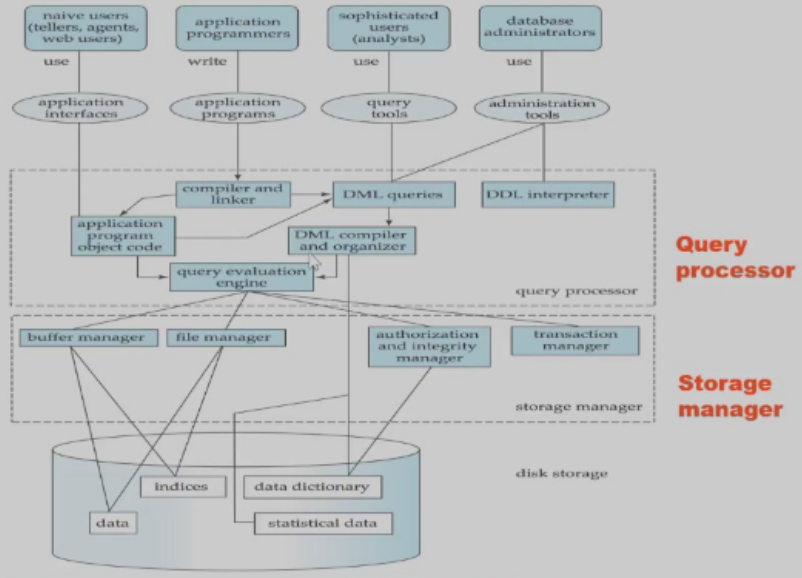
\includegraphics[width=0.309\textwidth]{DB1/Database System Internals}
    \caption{Database System Internals}
\end{figure}


\subsubsection{Application Architecture}

\subsection{History of Database Systems}

% Exercises: 1.7, 1.8, and 1.15 (see Page 32)